\setcounter{chapter}{6}
\setcounter{section}{0}
\part{ANEXOS}

\begin{figure}[H]
	\caption{Interfaz principal de aplicación demostrativa de la librería.}
	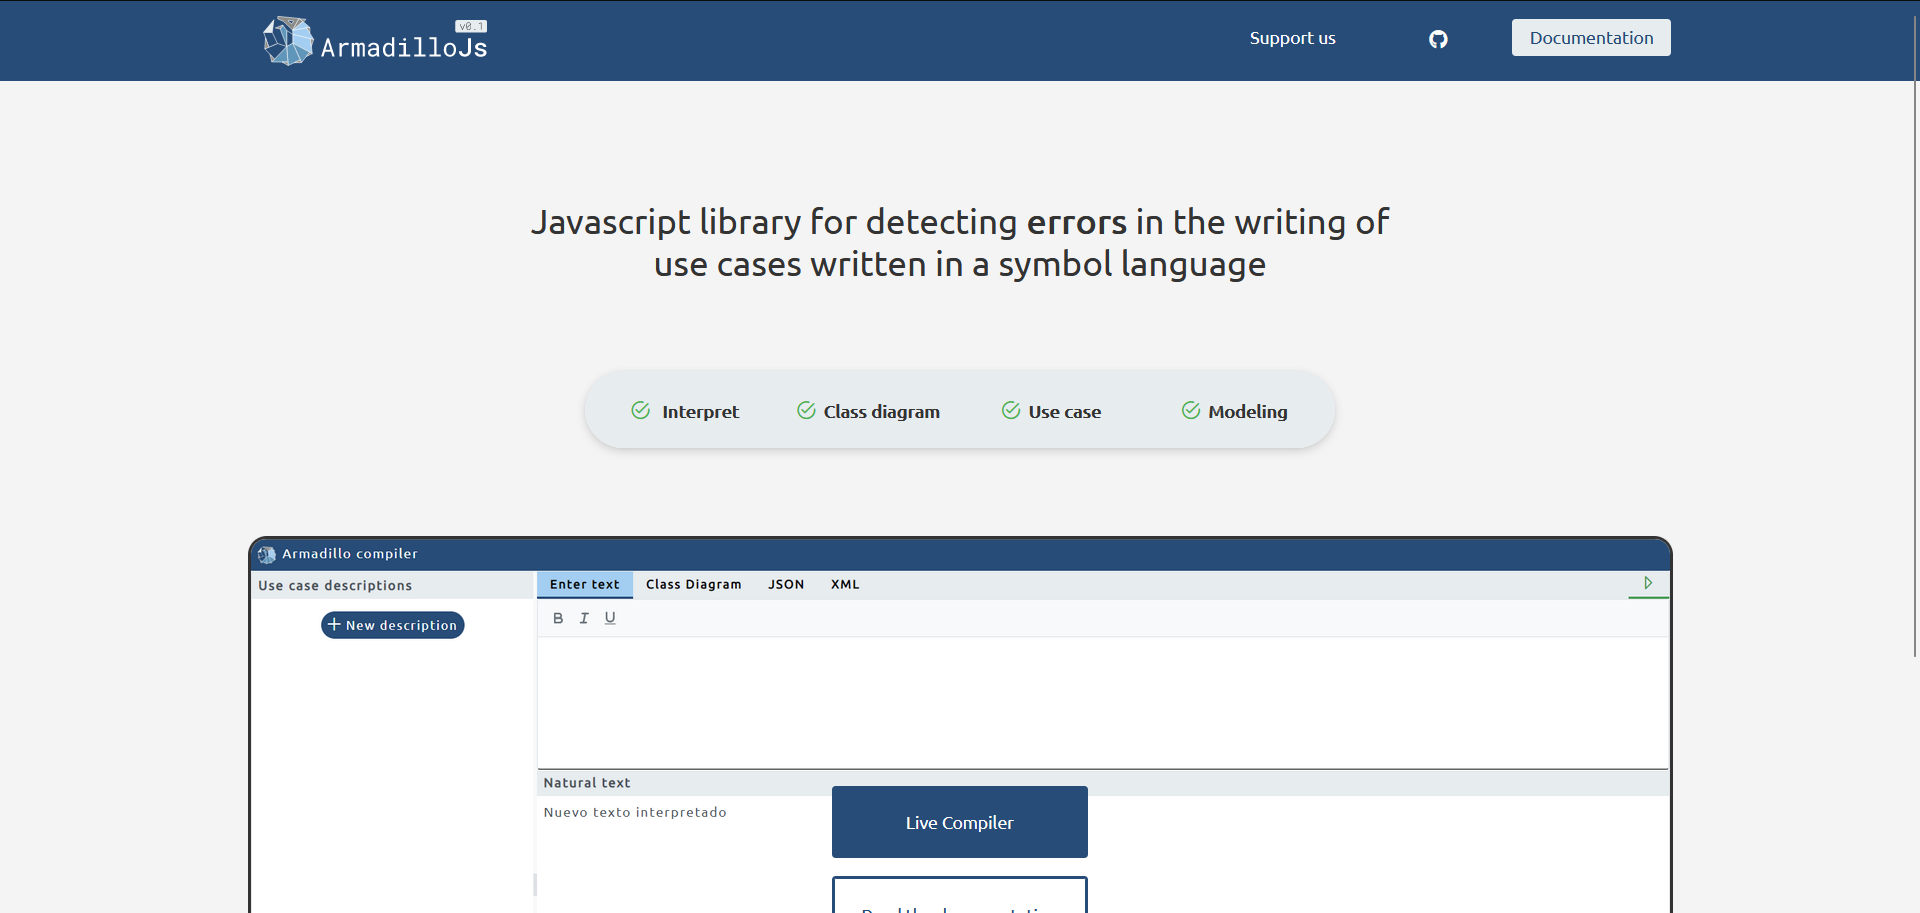
\includegraphics[width=15cm]{img/anexo1.png}
	\label{fig:anexo1}
	\textbf{\\ FUENTE: PROPIA \\ ELABORADO: DÚVAL CARVAJAL SUÁREZ}
\end{figure} 

\begin{figure}[H]
	\caption{Interfaz donde se ingresarán las descripciones de los casos de uso a interpretar.}
	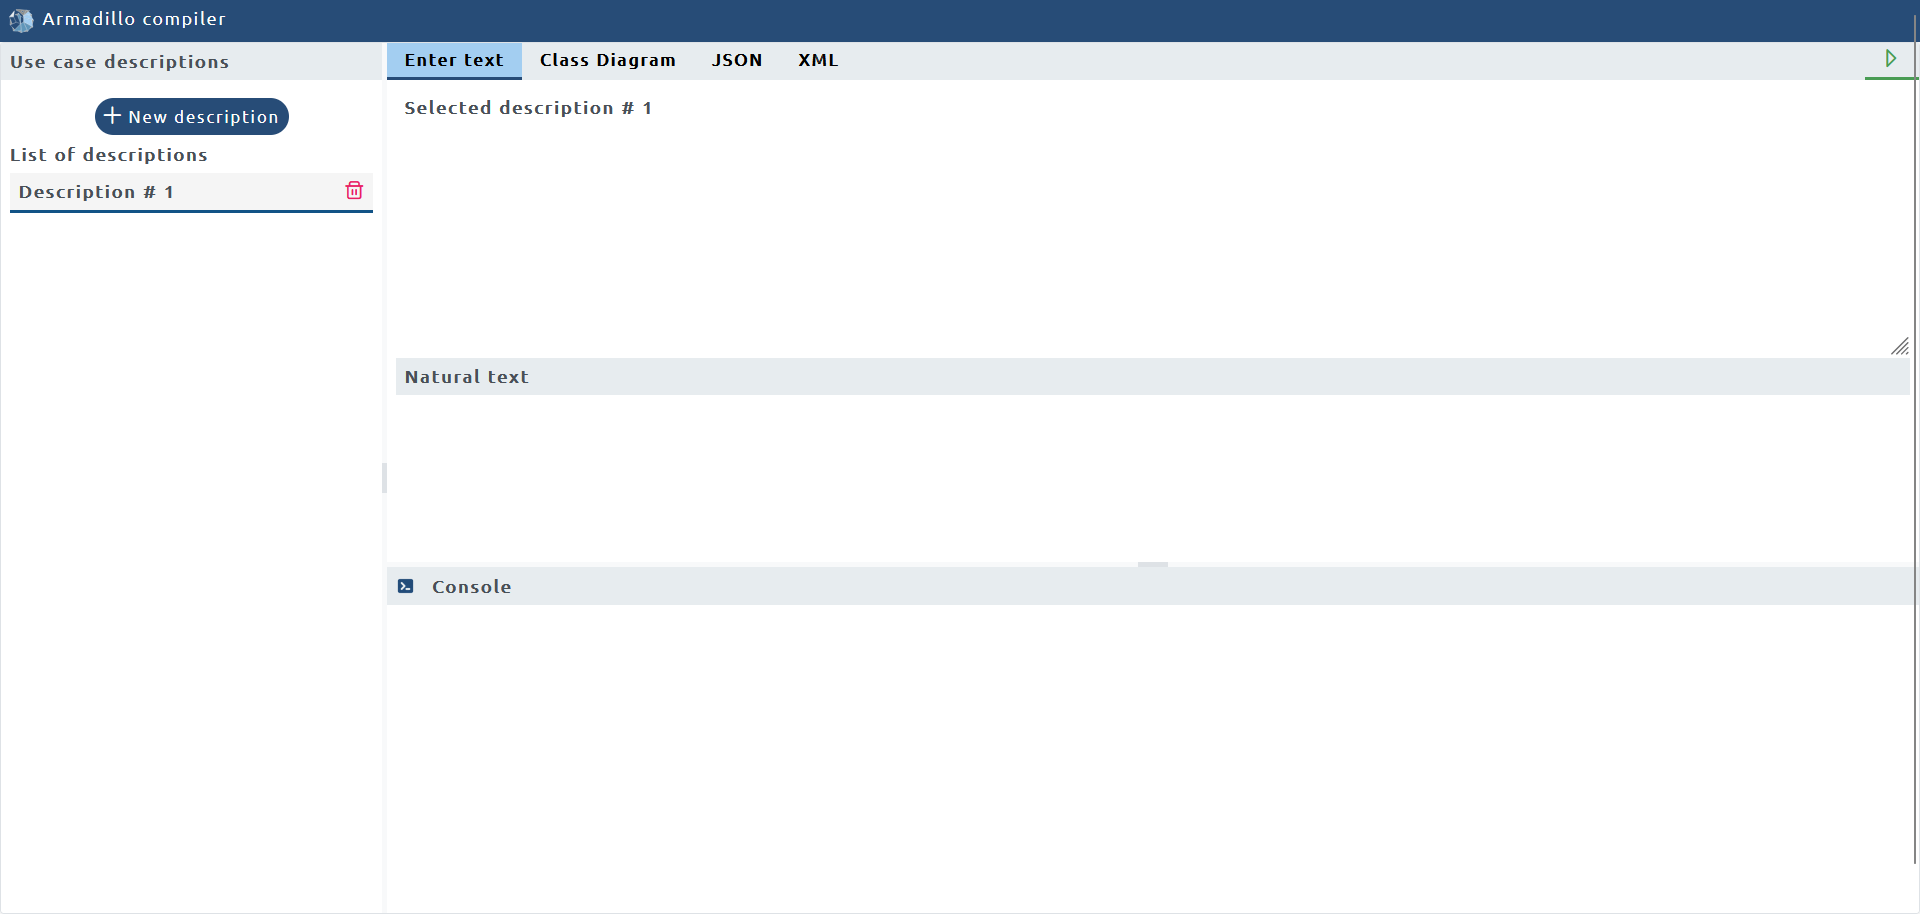
\includegraphics[width=15cm]{img/anexo2.png}
	\label{fig:anexo2}
	\textbf{\\ FUENTE: PROPIA \\ ELABORADO: DÚVAL CARVAJAL SUÁREZ}
\end{figure} 

\begin{figure}[H]
	\caption{Descripción del caso de uso interpretada con su respectiva retroalimentación.}
	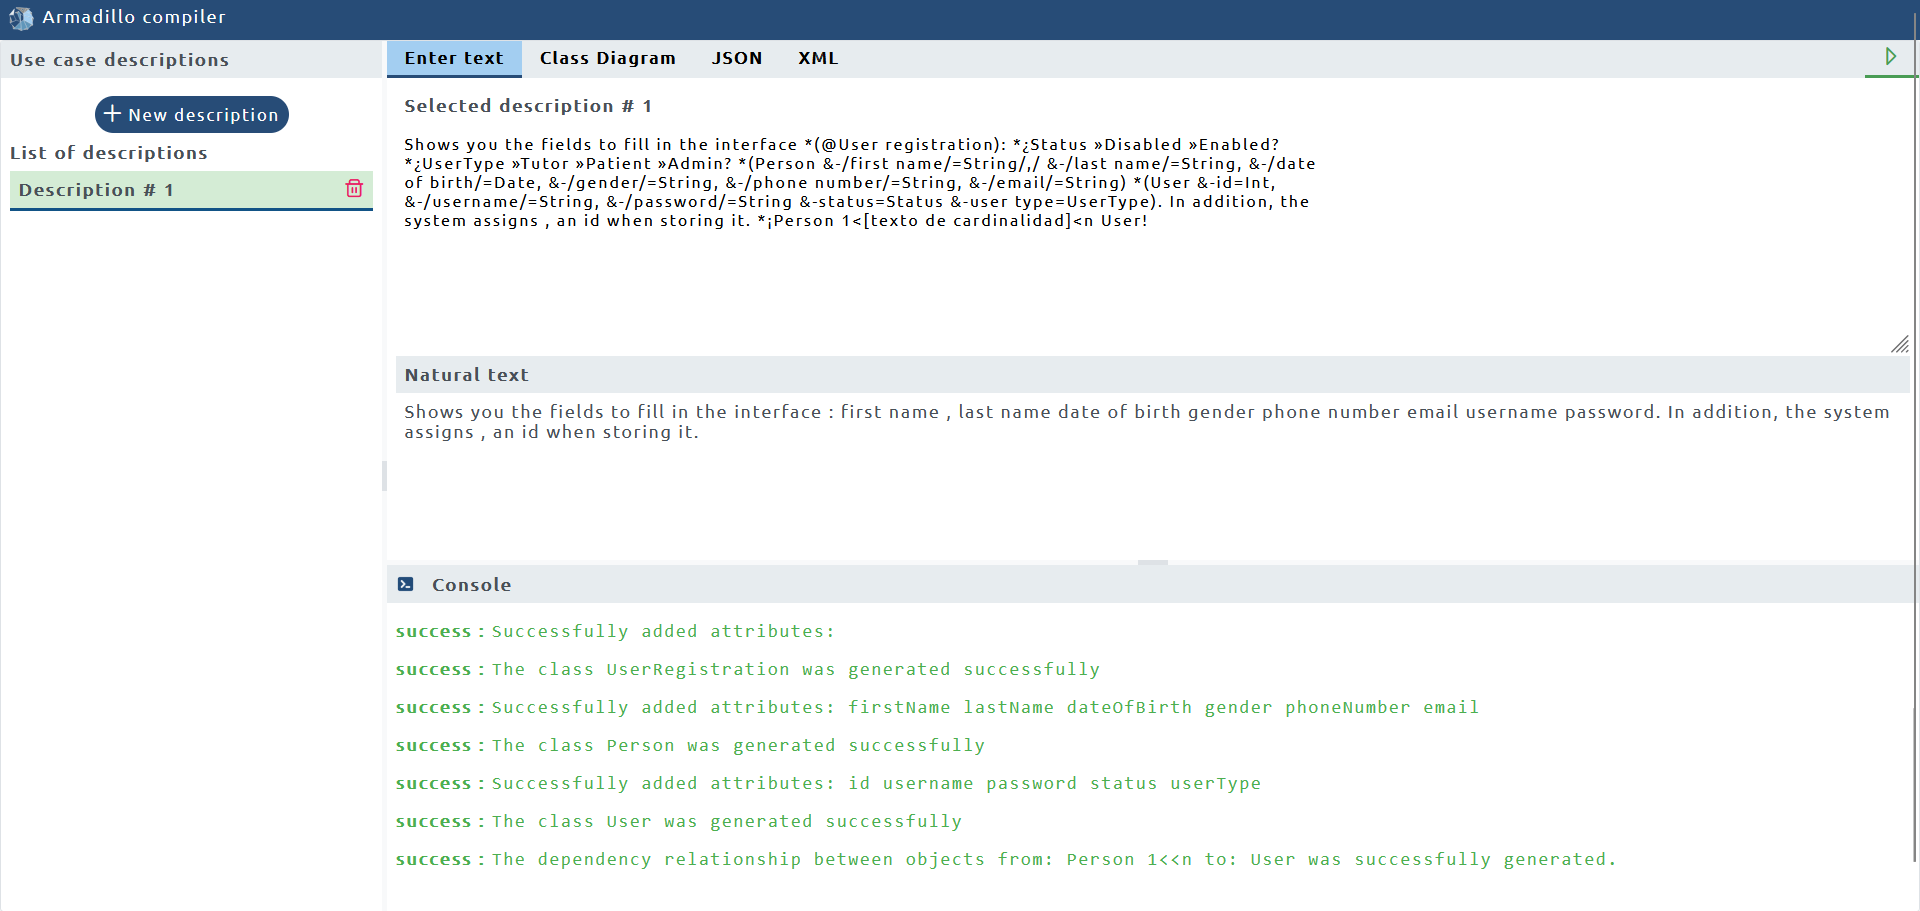
\includegraphics[width=15cm]{img/anexo3.png}
	\label{fig:anexo3}
	\textbf{\\ FUENTE: PROPIA \\ ELABORADO: DÚVAL CARVAJAL SUÁREZ}
\end{figure} 

\begin{figure}[H]
	\caption{Diagrama de clases generado por la librería usando una librería externa denominada jsUML2.}
	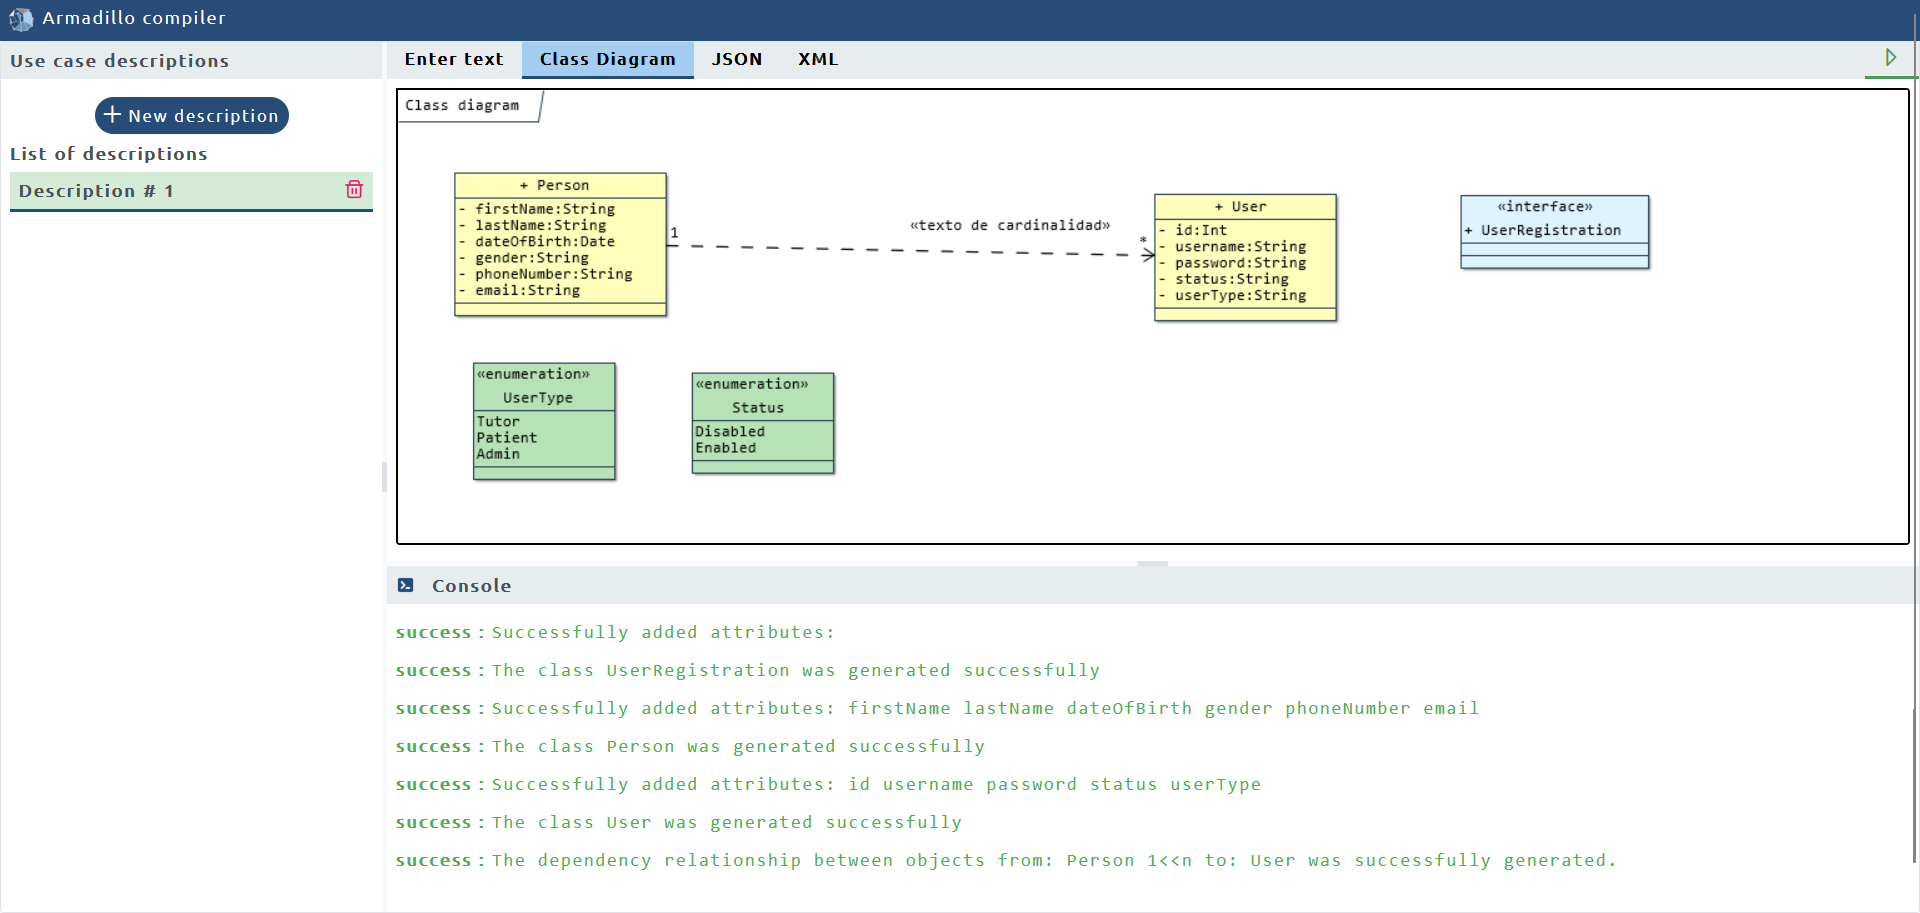
\includegraphics[width=15cm]{img/anexo4.png}
	\label{fig:anexo4}
	\textbf{\\ FUENTE: PROPIA \\ ELABORADO: DÚVAL CARVAJAL SUÁREZ}
\end{figure} 

\begin{figure}[H]
	\caption{Estructura JSON generada por la librería.}
	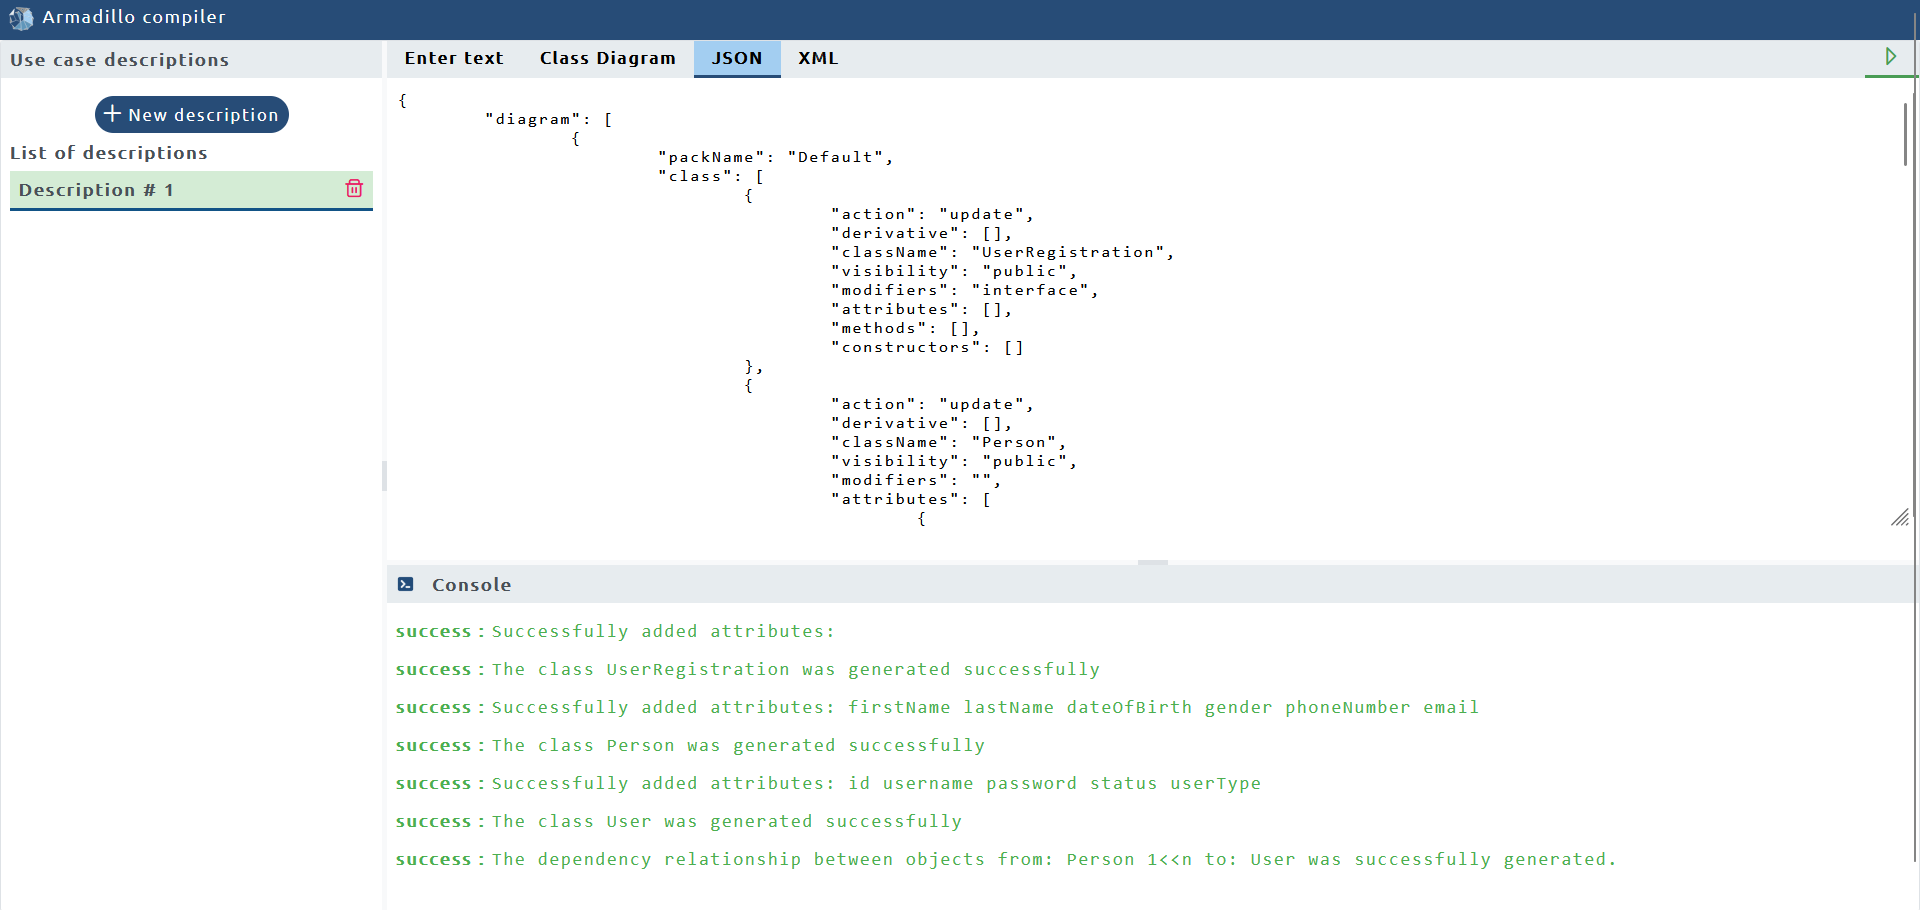
\includegraphics[width=15cm]{img/anexo5.png}
	\label{fig:anexo5}
	\textbf{\\ FUENTE: PROPIA \\ ELABORADO: DÚVAL CARVAJAL SUÁREZ}
\end{figure} 

\begin{figure}[H]
	\caption{XML generado por la librería.}
	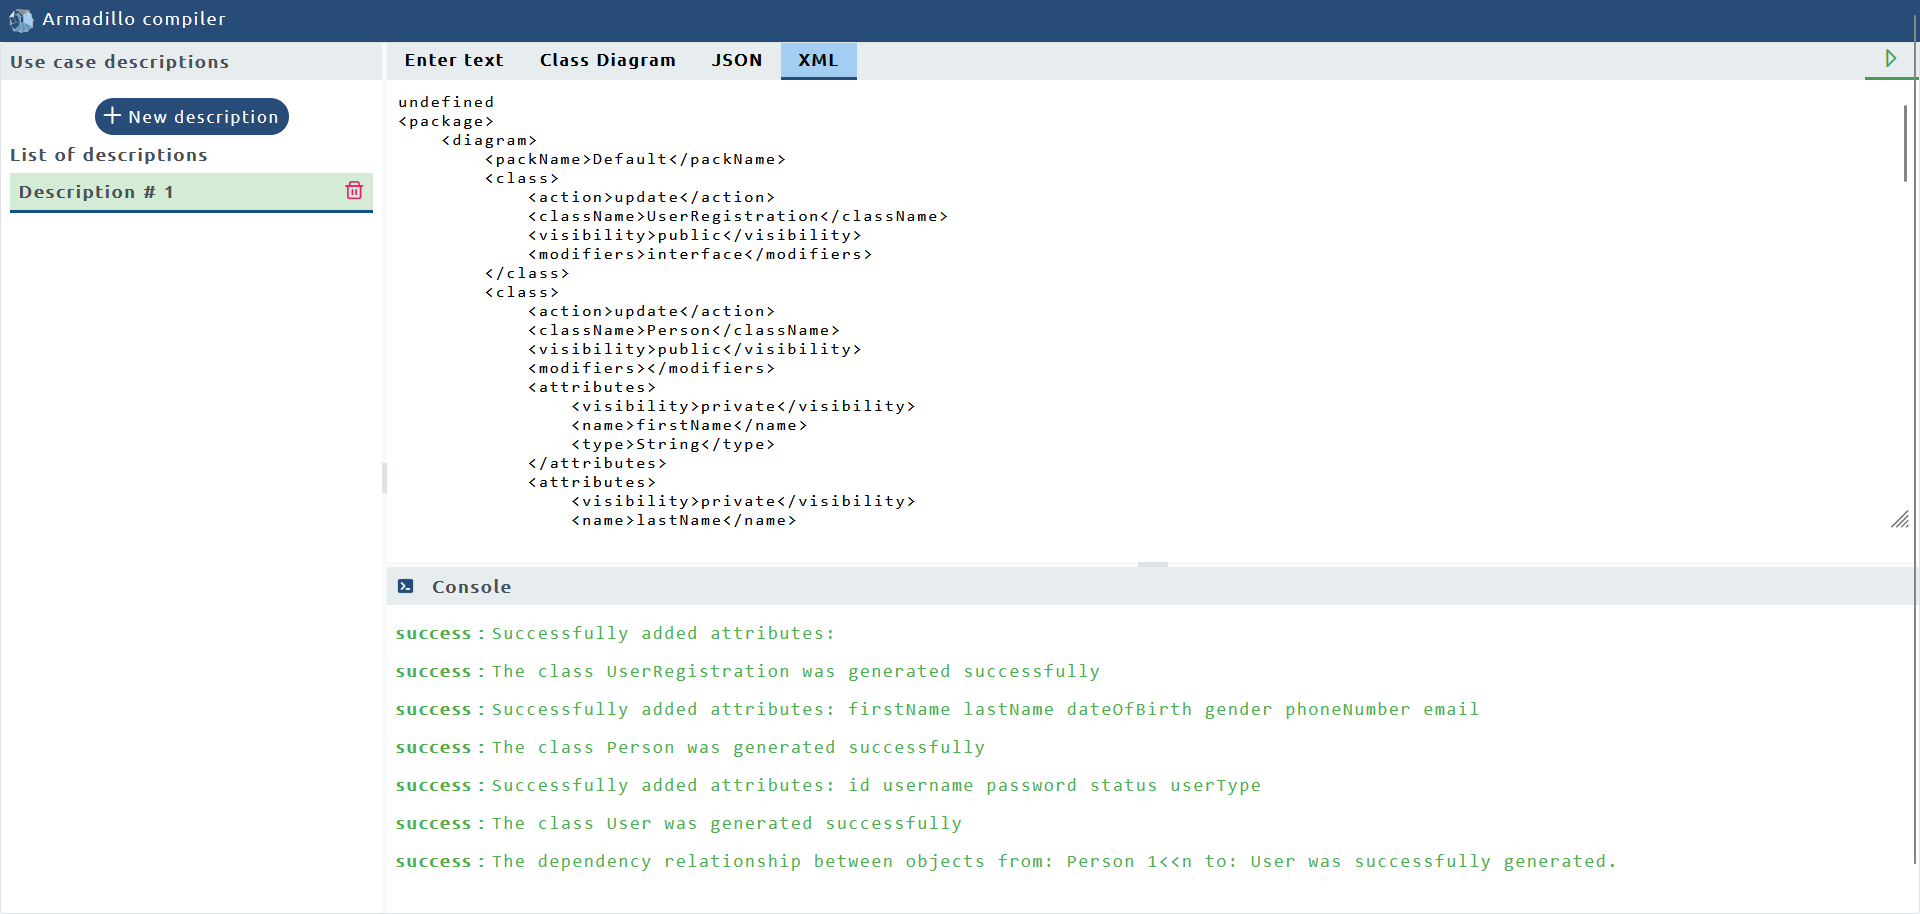
\includegraphics[width=15cm]{img/anexo6.png}
	\label{fig:anexo6}
	\textbf{\\ FUENTE: PROPIA \\ ELABORADO: DÚVAL CARVAJAL SUÁREZ}
\end{figure} 

\begin{figure}[H]
	\caption{Error detectado en la descripción del caso de uso}
	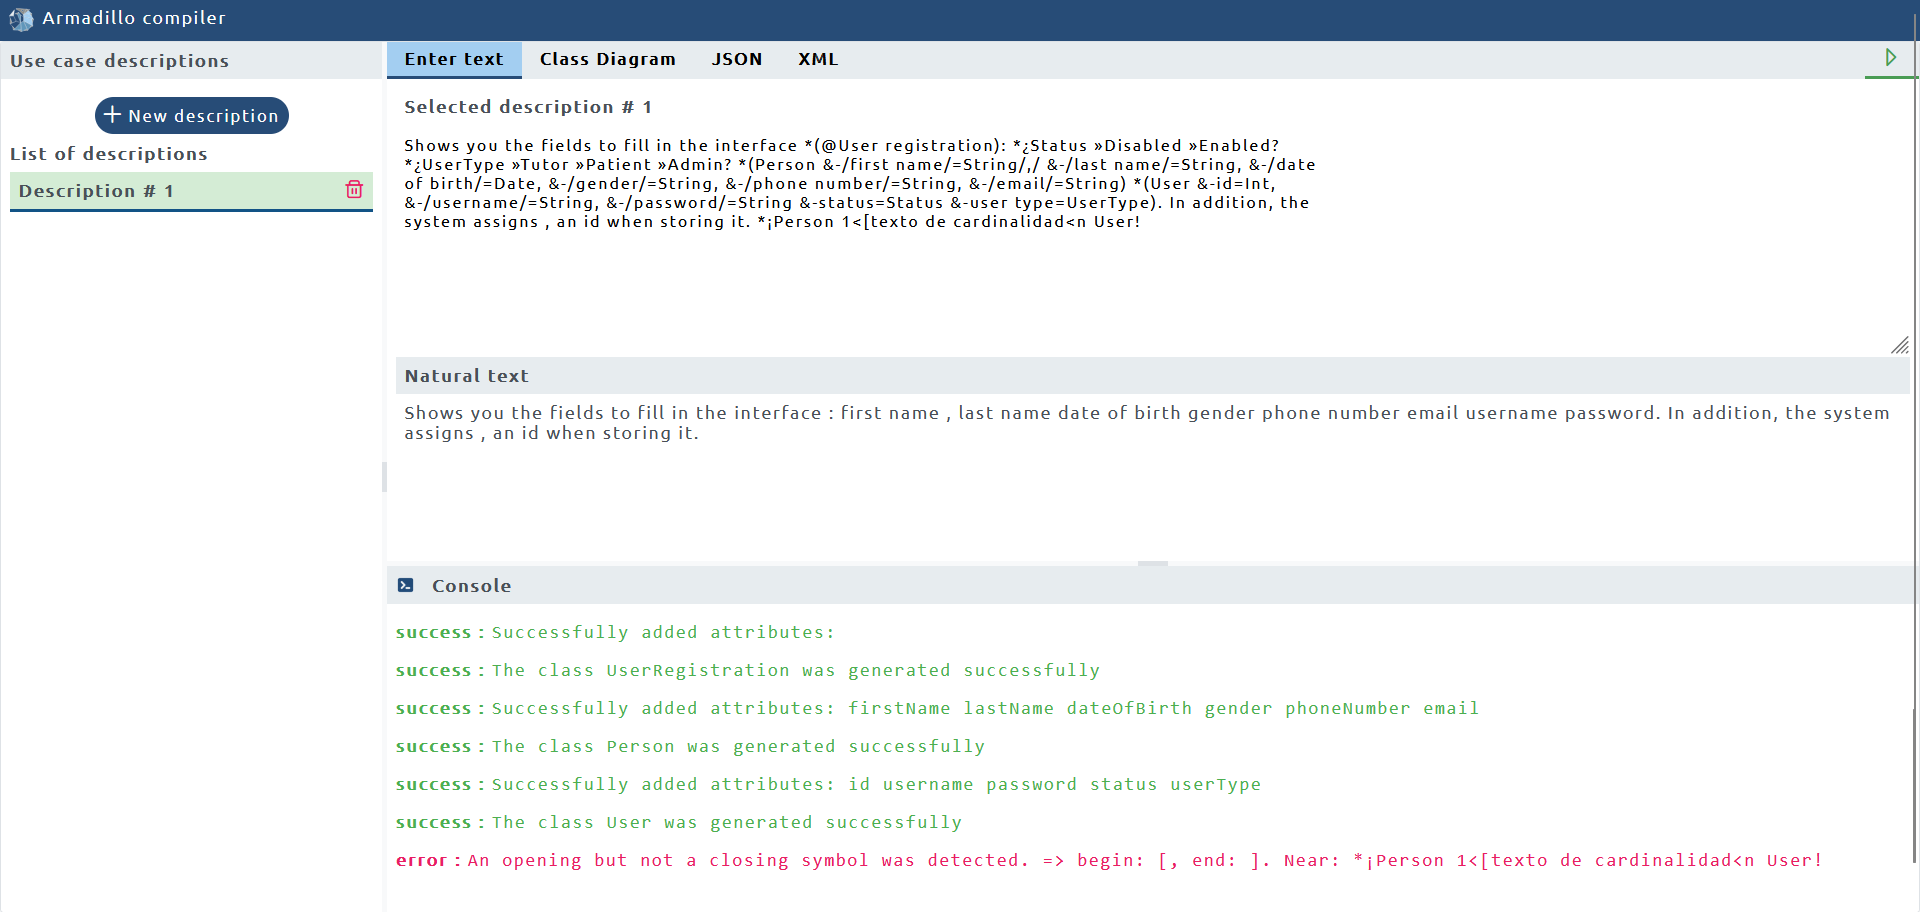
\includegraphics[width=15cm]{img/anexo7.png}
	\label{fig:anexo7}
	\textbf{\\ FUENTE: PROPIA \\ ELABORADO: DÚVAL CARVAJAL SUÁREZ}
\end{figure} 